% =========================================================
% Appendix-local full-width listing for ONE-COLUMN appendix
% =========================================================

\newenvironment{FullWidthListing}
{
  \begin{figure}[!htbp]
    \centering
    \begin{minipage}{0.97\linewidth}
    \vspace{4pt}
}
{
    \end{minipage}
  \end{figure}
  \FloatBarrier
}

% =========================================================
% APPENDIX: COMPLETE SYSTEM DOCUMENTATION (fixed)
% =========================================================
% \section{Complete System Documentation}
% \label{app:complete}

% Force single-column appendix environment
\AppendixOneColumn

\FloatBarrier

% ---- Appendix-wide spacing & box defaults ----
\captionsetup[figure]{skip=8pt}
\captionsetup[table]{skip=6pt}
\setlength{\textfloatsep}{12pt plus 2pt minus 2pt}
\setlength{\floatsep}{12pt plus 2pt minus 2pt}
\setlength{\intextsep}{12pt plus 2pt minus 2pt}

\tcbset{
  enhanced jigsaw,
  breakable,
  colback=gray!2,
  colframe=black!20,
  boxrule=0.4pt,
  left=6pt,right=6pt,top=6pt,bottom=6pt,
  before skip=10pt,
  after skip=14pt
}

\appendix
\onecolumn
\begin{center}
{\Large \textbf{APPENDIX}} \\[6pt]
\end{center}
% \twocolumn


% =========================================================
% SECTION A: USER INTERFACE AND SYSTEM ARCHITECTURE
% =========================================================
\section{User Interface and Runtime Architecture}
\label{app:interface}

\vspace{6pt}

\subsection{Player-Facing Interface Design}

\paragraph{Design Philosophy.}
Our UI emphasizes uninterrupted gameplay: player control remains primary. 
The right-hand chat rail presents all agent interactions, including 
\texttt{PlanPreview}, clarifying queries, live execution updates, and validator feedback. 
These elements surface inline and incrementally, avoiding disruptive modals. 
All interactions are timestamped and logged consistent with the 
Mineflayer-only evaluation policy. A video demonstration of this interaction flow is available at
\href{https://youtu.be/7hqQl9XhjAk}{\texttt{link}}.

\vspace{10pt}


\begin{figure}[!hbt]
  \centering
  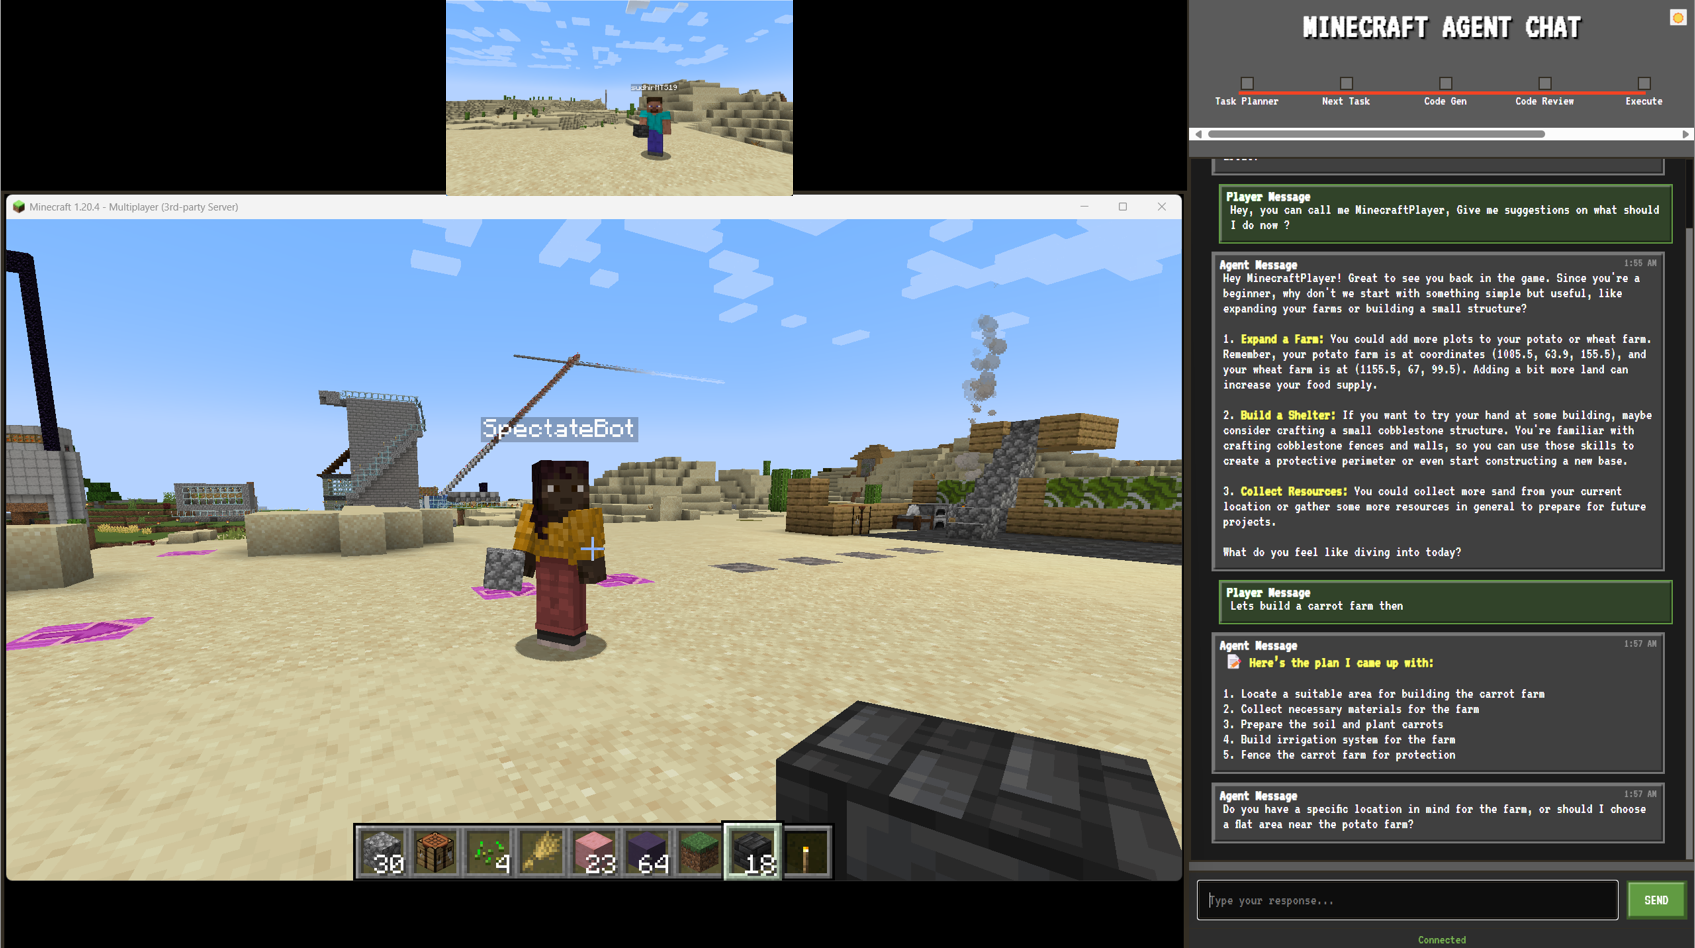
\includegraphics[width=\columnwidth]{Sections/Figures/user_interface.png}
  \caption{\textbf{Player interface for memory-grounded agent interaction.}
  \emph{Left:} Unobstructed main viewport with minimal spectator NPC.
  \emph{Right:} Lightweight side-rail chat for agent I/O plan previews, 
  clarification, validator summaries, and progress toasts.}
  \label{fig:ui-appx}
\end{figure}

\vspace{10pt}

\medskip


\subsection{Core Runtime Data Structures}
Below we document core runtime schemas used by the planner, memory, and validator modules. Each schema is designed for interpretability, serialization, and traceability across the pipeline.

\FloatBarrier
\vspace{6pt}

% -------------------------
% BotState Schema (table)
% -------------------------
% \subsubsection{BotState Schema}
\vspace{2pt}
\FloatBarrier

\begin{table}[!htbp]
  \centering
  \caption{\texttt{BotState}: snapshot of world and agent state at a given tick.}
  \label{tab:botstate}
  \begin{tabularx}{\linewidth}{@{} l l X @{}}
    \toprule
    \textbf{Field} & \textbf{Type} & \textbf{Description} \\
    \midrule
    time & int & In-game tick count when captured. \\
    position & Position & Absolute world coordinates \((x,y,z)\). \\
    health, hunger & int & Current health and hunger values. \\
    nearby\_blocks & List\textless{}str\textgreater{} & Surrounding block types in range. \\
    equipment & List\textless{}str\textgreater{} & Equipped items (tools, armor). \\
    inventory & Inventory & Complete item inventory with counts. \\
    chests & List\textless{}str\textgreater{} & Recently seen or accessed chest locations. \\
    movement & Movement & Current movement goal and state. \\
    nearby\_entities & List\textless{}Entity\textgreater{} & Visible entities with metadata. \\
    recent\_chat & List\textless{}str\textgreater{} & Recent messages in local chat. \\
    active\_effects & List\textless{}str\textgreater{} & Active potion/status effects. \\
    environment & Environment & Environmental context (biome, weather, time). \\
    target\_block & Optional\textless{}str\textgreater{} & Current interaction target (if any). \\
    \bottomrule
  \end{tabularx}
\end{table}

\FloatBarrier
\vspace{8pt}

% -------------------------
% TaskModel Schema
% -------------------------
% \subsubsection{TaskModel Schema}
\vspace{2pt}
\FloatBarrier

\begin{table}[!htbp]
  \centering
  \caption{\texttt{TaskModel}: normalized subtask representation.}
  \label{tab:taskmodel}
  \begin{tabularx}{\linewidth}{@{} l l X @{}}
    \toprule
    \textbf{Field} & \textbf{Type} & \textbf{Description} \\
    \midrule
    index & int & Unique index within plan. \\
    subtask & str & Natural language description. \\
    dependencies & List\textless{}int\textgreater{} & Indices of prerequisite subtasks. \\
    parameters & Any & Arguments required for execution. \\
    status & str & Execution state: \texttt{pending} \(|\) \texttt{in-progress} \(|\) \texttt{completed}. \\
    clarifying\_questions & List\textless{}str\textgreater{} & Outstanding disambiguation questions. \\
    success\_criteria & str & Machine-checkable completion condition. \\
    \bottomrule
  \end{tabularx}
\end{table}

\FloatBarrier
\vspace{8pt}

% -------------------------
% ValidationOutput Schema
% -------------------------
% \subsubsection{ValidationOutput Schema}
\vspace{2pt}
\FloatBarrier

\begin{table}[!htbp]
  \centering
  \caption{\texttt{ValidationOutput}: task evaluation with reasoning.}
  \label{tab:validation}
  \begin{tabularx}{\linewidth}{@{} l l X @{}}
    \toprule
    \textbf{Field} & \textbf{Type} & \textbf{Description} \\
    \midrule
    success, failure & Optional\textless{}str\textgreater{} & Human-readable explanation. \\
    state\_changes & List\textless{}StateChange\textgreater{} & Key in-world deltas. \\
    chat\_insights & List\textless{}ChatMessage\textgreater{} & Relevant parsed chat excerpts. \\
    suggestions & Optional\textless{}str\textgreater{} & Repair/retry recommendations. \\
    question\_for\_player & Optional\textless{}str\textgreater{} & Clarification prompt if ambiguous. \\
    is\_task\_completed & bool & Binary task verdict. \\
    final\_result & Optional\textless{}str\textgreater{} & Validator's reasoning summary. \\
    confidence\_score & int & Certainty level \([0,10]\). \\
    \bottomrule
  \end{tabularx}
\end{table}

\FloatBarrier
\vspace{10pt}

% -------------------------
% Pydantic Implementation
% -------------------------
\newpage
\subsection{Pydantic Schema Definitions}
\label{app:pydantic}
\vspace{4pt}
\FloatBarrier

\begin{FullWidthListing}
\caption{Production runtime schemas in Pydantic.}
\label{lst:schemas}
\begin{lstlisting}[language=Python]
class BotState(BaseModel):
    """Agent state snapshot"""
    time: int
    position: Position
    health: int
    hunger: int
    nearby_blocks: List[str]
    equipment: List[str]
    inventory: Inventory
    chests: List[str]
    movement: Movement
    nearby_entities: List[Entity]
    recent_chat: List[str]
    active_effects: List[str]
    environment: Environment
    target_block: Optional[str]

class TaskModel(BaseModel):
    """Structured subtask with dependencies"""
    index: int
    subtask: str
    dependencies: List[int] = []
    parameters: Any = {}
    status: str = "pending"
    clarifying_questions: List[str] = []
    success_criteria: str

class ValidationOutput(BaseModel):  
    """Validator outputs"""
    success: Optional[str]
    failure: Optional[str]
    state_changes: List[StateChange] = []
    chat_insights: List[ChatMessage] = []
    suggestions: Optional[str]
    question_for_player: Optional[str]
    is_task_completed: bool
    final_result: Optional[str]
    confidence_score: int
\end{lstlisting}
\end{FullWidthListing}

\clearpage

% =========================================================
% SECTION B: TASK PLANNING PROMPT TEMPLATES
% =========================================================
\section{Task Planning and Replanning Prompts}
\label{app:planning}

\vspace{10pt}

\subsection{Initial Task Planning}

\vspace{10pt}

\subsubsection{System Prompt: Initial Task Planner}


\begin{tcolorbox}[title=System Prompt: Initial Task Planner]
You are an advanced \textbf{Minecraft AI Task Planner}, responsible for generating structured and executable task plans for a personalized Minecraft assistant. You use the \textbf{Mineflayer API} to ensure tasks are well-defined, achievable, and optimized based on real-time game conditions and user preferences.

\textbf{Core Responsibilities:}
\begin{itemize}[leftmargin=*]
  \item Break down high-level user tasks into structured, sequential subtasks.
  \item Minimize unnecessary clarifications via bot state and user context.
  \item Generate plans that are executable within current game conditions.
  \item \textbf{Never} modify previously completed tasks during replanning.
\end{itemize}
\end{tcolorbox}

\begin{lstlisting}[style=json,caption={Expected JSON output for the initial task planner.}]
{
  "task_plan": [
    {
      "index": 1,
      "subtask": "Clear, actionable description",
      "dependencies": [],
      "parameters": {},
      "status": "pending",
      "clarifying_questions": [],
      "success_criteria": "Measurable completion condition"
    }
  ]
}
\end{lstlisting}

% =========================================================
% SECTION C: CLARIFICATION AND FEEDBACK PROMPTS
% =========================================================
\section{Clarification and Feedback Management}
\label{app:clarification}

\vspace{10pt}

\subsection{Subtask Clarification System}

\vspace{10pt}

\begin{tcolorbox}[title=System Prompt: Subtask Clarification]
Given a task with outstanding clarifying questions in JSON, generate the missing information while preserving all existing fields.
\end{tcolorbox}

\begin{lstlisting}[style=json,caption={Example task requiring clarification.}]
{
  "index": 2,
  "subtask": "Retrieve a sword from the chest",
  "parameters": {"item_name": "sword"},
  "clarifying_questions": ["What type of sword do you need?"]
}
\end{lstlisting}

\begin{lstlisting}[style=json,caption={Clarification response example.}]
[
  {
    "question": "What type of sword do you need?",
    "answer": "diamond_sword"
  }
]
\end{lstlisting}

% =========================================================
% SECTION D: VALIDATION AND CODE GENERATION
% =========================================================
\section{Validation, Code Generation, and System Updates}
\label{app:validation}

\vspace{10pt}

\subsection{Subtask Validation System}

\begin{tcolorbox}[title=System Prompt: Subtask Validator]
You are a \textbf{Validation AI Agent} responsible for evaluating a Minecraft bot's task execution via world-state analysis and producing structured reports.
\end{tcolorbox}

\subsection{Player Landmark Tracking System}

\begin{lstlisting}[style=json,caption={Landmark update schema.}]
{
  "landmarks": {
    "weapon storage": {
      "coordinates": [x, y, z],
      "radius": 6
    }
  }
}
\end{lstlisting}

\subsection{Code Generation and Review Examples}

\begin{lstlisting}[style=json,caption={Code generation output example.}]
{
  "code": "async function task(bot) { /* implementation */ }"
}
\end{lstlisting}

\begin{lstlisting}[style=json,caption={Code review output example.}]
{
  "valid": true,
  "confidence": 0.9,
  "comments": [
    {"line": 5,  "comment": "Use mineBlock() instead of bot.dig()"},
    {"line": 12, "comment": "Add null check for bot.inventory"}
  ]
}
\end{lstlisting}


\clearpage
% =========================================================
% SECTION E: TASK CORPUS AND EVALUATION DATA (MineNPC-Task)
% =========================================================

% --- spacing helpers (safe to define once; no-ops if already present)
\providecommand{\appxsep}{\vspace{0.8\baselineskip}}
\providecommand{\appxsmallsep}{\vspace{0.45\baselineskip}}

% Lists a bit airier than default but still compact.
\setlist[itemize]{leftmargin=*, topsep=4pt, itemsep=2pt}
\setlist[enumerate]{leftmargin=*, topsep=4pt, itemsep=2pt}

% Friendlier tcolorboxes with breathing room
\tcbset{
  appxbox/.style={
    colback=gray!2, colframe=black!15,
    enhanced, sharp corners,
    boxsep=1ex, left=1.2ex, right=1.2ex, top=0.8ex, bottom=0.8ex,
    before skip=12pt, after skip=14pt, breakable
  }
}

\BackToTwoColumn

\section{\textsc{MineNPC-Task} and Subtask Breakdown}
\label{app:tasksuite}


\appxsmallsep
The following \textbf{44 tasks} constitute the \emph{complete} \textsc{MineNPC-Task} suite used in our study. They were elicited from expert co-play rather than synthesized prompts, span multiple gameplay domains, and define the benchmark workload for evaluating agents under our bounded-knowledge policy.

\appxsep
\subsection{High-Level Task Categories in \textsc{MineNPC-Task}}

\subsubsection{Resource Collection and Mining}
\begin{itemize}
  \item Mine and collect cobblestones and deliver them.
  \item Mine cobblestones starting from specific coordinates (1145, 58, 56).
  \item Use pickaxe to mine 20 blocks of cobblestone in front of player.
  \item Use golden pickaxe to mine 5 cobblestone blocks.
  \item Mine coal nearby using diamond pickaxe.
  \item Continue mining 4 coal blocks, then deliver cobblestone and coal.
  \item Mine 16 stones from designated spot, find and mine 4 coal blocks.
  \item Mine iron ore for the player.
  \item Take iron pickaxe and get at least 10 coal blocks.
  \item Drop 5 cobblestones in front of player.
  \item Give 4 cobblestones to player.
  \item Harvest oak logs (at least 20 blocks) using an axe.
\end{itemize}

\appxsmallsep
\subsubsection{Tool and Equipment Management}
\begin{itemize}
  \item Pick up a pickaxe from the pickaxe chest.
  \item Get a pickaxe from the chest at the best entrance.
  \item Get a pickaxe from the chest at the mine.
  \item Grab an iron pickaxe from the chest at \texttt{ChestEntrance}.
  \item Bring iron pickaxe from \texttt{iron\_pickaxe\_chest}.
  \item Get iron pickaxe from ``Storage''.
  \item Come to player and drop the coal.
  \item Give cobblestone that was mined.
\end{itemize}

\appxsmallsep
\subsubsection{Agriculture and Food}
\begin{itemize}
  \item Harvest 5 wheat.
  \item Harvest wheat and craft bread.
  \item Collect wheat and make 3 pieces of bread.
  \item Harvest wheat and craft 3 pieces of bread if needed.
  \item Collect 18 wheat blocks.
  \item Help plant more seeds.
  \item Go to ``Farm'' to harvest wheat for 2 bread.
  \item Walk around and pick up all harvested wheat.
\end{itemize}

\appxsmallsep
\subsubsection{Construction and Building}
\begin{itemize}
  \item Build a pyramid from sand (5$\times$5 base).
  \item Build a simple house with roof at \texttt{build\_spot}.
  \item Collect dirt and build a dirt house.
  \item Build walls for the house.
  \item Build a wall 10 blocks long and 2 blocks high next to house.
  \item Make a 4$\times$2 vertical wall at specified coordinates.
  \item Decorate house with blue stained glass at specific coordinates.
\end{itemize}

\appxsmallsep
\subsubsection{Crafting and Processing}
\begin{itemize}
  \item Turn stripped oak logs into planks, then into stairs.
  \item Come to location and craft stairs.
  \item Collect materials from preferred building list.
\end{itemize}

\appxsmallsep
\subsubsection{Storage and Inventory}
\begin{itemize}
  \item Put wood-related blocks into the chest in front of player.
  \item Get stained glass from design chest (10 blocks).
  \item Give 5 pieces of magenta stained glass and 2 pieces of redstone block.
  \item Bring 25 blocks of stripped cherry wood and 4 lanterns.
  \item Give all cherry wood and lanterns.
  \item Drop brain coral block, exposed copper, and terracotta.
\end{itemize}

\FloatBarrier
\appxsep
\subsection{Full Subtask Decomposition for \textsc{MineNPC-Task}}

\begin{small}
\begin{enumerate}
  \item Mine cobblestone.
  \item Mine cobblestone starting from specified coordinates.
  \item Navigate to the nearest chest.
  \item Locate and verify crafting table at \texttt{wheat\_farm}.
  \item Locate the nearest lava source.
  \item Walk around to find a nearby crafting table.
  \item Locate a nearby tree to collect wood.
  \item Navigate to the cave or mine shaft.
  \item Move to the chest in front of the player.
  \item Move to the chest location.
  \item Locate player's boat nearby.
  \item Return to user with collected items.
  \item Navigate to the Pickaxe chest.
  \item Go to the starting coordinate for mining.
  \item Find the nearest chest.
  \item Navigate to the coal site.
  \item Go to player \texttt{ThorThunder92}.
  \item Locate the player to give wheat.
  \item Navigate to the closest coal ore block.
  \item Travel to \texttt{build\_spot}.
  \item Navigate to \texttt{ChestEntrance}.
  \item Navigate to the \texttt{wheatFarm} location.
  \item Navigate to a dirt-rich area.
  \item Navigate to the Storage location.
  \item Locate a cave or mine shaft.
  \item Travel to Farm.
  \item Move around the farm area to locate dropped wheat.
  \item Go to the farm area.
  \item Approach the nearest player.
  \item Locate oak trees in the surrounding area.
  \item Move to the nearest oak tree.
  \item Return to the original position or safe location.
  \item Locate the user.
  \item Navigate to the treasure box location.
  \item Navigate to the wood storage area.
  \item Go to the mine.
  \item Locate the nearest cobblestone block.
  \item Move to the cobblestone block.
  \item Locate the nearest player to hand over cobblestone.
  \item Move to the nearest player.
  \item Navigate to the wheat farm.
  \item Locate player ``ThorThunder92''.
  \item Go to the design storage chest.
  \item Locate the design storage chest.
  \item Locate the block storage chest.
  \item Navigate to utilities area.
  \item Go to the block storage.
  \item Go to the chest in the utilities.
  \item Move to specified coordinates.
  \item Go to the chest location.
  \item Harvest 5 wheat.
  \item Mine 16 cobblestone.
  \item Collect nearby wheat items.
  \item Search for and pick up an axe.
  \item Collect stripped cherry wood.
  \item Collect stripped cherry wood from wood storage.
  \item Gather 5 pieces of glass.
  \item Collect 10 blocks of stained glass from the chest.
  \item Collect 2 pieces of redstone block from block storage.
  \item Collect additional wheat.
  \item Collect dropped wheat.
  \item Collect material for building walls.
  \item Collect 32 terracotta blocks from chest.
  \item Collect enough building material for the wall.
  \item Explore to find cobblestone.
  \item Mine cobblestone until 20 are collected.
  \item Collect wheat from the ripened wheat farm.
  \item Collect sufficient sand for pyramid construction.
  \item Gather required materials for pyramid.
  \item Get 18 items of wheat from wheat crops.
  \item Harvest matured wheat.
  \item Mine the coal ore block.
  \item Search for iron ore.
  \item Harvest wheat from the farm.
  \item Harvest oak logs using stone axe.
  \item Collect dirt blocks.
  \item Pick up the golden pickaxe from treasure box.
  \item Collect 25 blocks of stripped cherry wood.
  \item Collect 4 lanterns.
  \item Collect 5 pieces of magenta stained glass.
  \item Mine 3 blocks of coal from identified deposits.
  \item Mine 5 cobblestone blocks using golden pickaxe.
  \item Check for mature wheat and harvest.
  \item Retrieve 64 green glazed terracotta from chest.
  \item Locate and open the chest.
  \item Open the chest and collect 32 terracotta blocks.
  \item Open the Pickaxe chest.
  \item Open the chest at \texttt{ChestEntrance}.
  \item Open the treasure box.
  \item Open the design storage chest.
  \item Check wood storage for stripped cherry wood.
  \item Check style storage for lanterns.
  \item Collect brain coral block from sea or storage.
  \item Gather exposed copper from storage or crafting.
  \item Gather magenta stained glass from storage.
  \item Check the chest for blue or green colored blocks.
  \item Check for blue terracotta block.
  \item Craft 2 breads from harvested wheat.
  \item Craft bread.
  \item Use the nearby crafting table to craft bread.
  \item Craft planks from available logs.
  \item Craft a stone axe using available material.
  \item Craft bread (from farm wheat).
  \item Craft oak planks from stripped oak logs.
  \item Craft bread using wheat.
  \item Craft 3 bread using collected wheat.
  \item Load sand into the located furnace.
  \item Add fuel to the furnace to start smelting.
  \item Retrieve 3 glass blocks from the furnace.
  \item Locate a nearby furnace.
  \item Identify the furnace location in front of the bot.
  \item Craft planks from available logs.
  \item Check the inventory for oak logs.
  \item Ensure crafting table is properly placed or accessible.
  \item Locate the seed dropped by the user.
  \item Plant wheat seeds within a radius of 10 blocks.
  \item Identify all farmland blocks within 10-block radius.
  \item Plant wheat seeds on all identified farmland blocks.
  \item Locate seeds in the inventory.
  \item Select building material from inventory.
  \item Select diamond pickaxe from inventory.
  \item Retrieve \texttt{blue\_stained\_glass} from inventory.
  \item Verify iron pickaxe in the inventory.
  \item Check for inventory.
  \item Select 4 cobblestones from inventory.
  \item Retrieve cobblestone from inventory.
  \item Check inventory for diamond pickaxe.
  \item List all items from inventory.
  \item Locate golden pickaxe in inventory or known chest.
  \item Identify wood-related items in the inventory.
  \item Build 4 by 2 blocks.
  \item Select current location as pyramid build location.
  \item Select suitable location to build the pyramid.
  \item Build base layer of pyramid with sand.
  \item Lay the foundation layer of 5$\times$5.
  \item Lay the second layer of 4$\times$4.
  \item Lay the third layer of 3$\times$3.
  \item Lay the fourth layer of 2$\times$2.
  \item Place the final block at the top.
  \item Begin constructing the house framework using planks.
  \item Construct the walls of the dirt house.
  \item Find a suitable location for building the dirt house.
  \item Locate house to start decorating.
  \item Place \texttt{blue\_stained\_glass} at specified coordinates.
  \item Place blocks to ascend to the surface.
  \item Determine location of the house.
  \item Return to X and transfer coal.
  \item Transfer 4 cobblestones to the nearest player.
  \item Retrieve a pickaxe from the chest.
  \item Give the cobblestone to the player.
  \item Return to the player and give the bread.
  \item Give 5 cobblestones to the closest player.
  \item Return to the user and give cobblestones.
  \item Transfer coal to the player \texttt{ThorThunder92}.
  \item Bring an iron pickaxe from \texttt{iron\_pickaxe\_chest}.
  \item Return to the player and present the iron pickaxe.
  \item Transfer coal and cobblestone to Rene.
  \item Adjust pathfinding to get close to X and deliver iron pickaxe.
  \item Return to the user and deliver the iron pickaxe.
  \item Punch the player.
  \item Drop oak stair in front of the bot.
  \item Drop the terracotta.
  \item Drop the brain coral block.
  \item Drop the exposed copper.
  \item Drop 5 cobblestones in front of the player.
  \item Deliver the 3 bread to the player.
  \item Give all cherry wood and lanterns to the player.
  \item Retrieve the gold pickaxe from the chest.
  \item Bring the golden pickaxe to the user.
  \item Transfer the 64 green glazed terracotta to player.
  \item Locate the chest containing the stone pickaxe.
  \item Retrieve a pickaxe from the Pickaxe chest.
  \item Retrieve an iron pickaxe from the chest.
  \item Locate the nearest chest.
  \item Retrieve diamond pickaxe from utilities area chest.
  \item Check if wheat farm has sufficient mature wheat.
  \item Check the maturity of wheat crops at ripened wheat farm.
  \item Move to the starting point for wheat collection.
  \item Align with mature wheat crop.
  \item Ensure the farming tool is functional.
  \item Locate a sand collection area.
  \item Navigate to pyramid location.
  \item Look around and identify all visible coal ore blocks.
  \item Attempt to harvest additional wheat.
  \item Identify matured wheat crops in nearby farmland.
  \item Locate and open the chest.
  \item Verify if the chest at the mine contains an iron pickaxe.
  \item Retrieve an iron pickaxe from the chest.
  \item Return to the player and give the iron pickaxe.
  \item Use iron pickaxe to mine 20 cobblestone blocks.
  \item Check for lime terracotta block.
  \item Retrieve the diamond pickaxe from the chest.
  \item Locate nearby coal deposits.
  \item Navigate to a mining area where cobblestone can be found.
  \item Locate the closest player entity.
  \item Go to the wheat farm to harvest wheat.
  \item Go to the location of the house.
  \item Go to the storage chest containing terracotta blocks.
  \item Locate the green glazed terracotta in design storage chest.
  \item Locate player to deliver the item.
  \item Move to the designated wall construction area next to the house.
  \item Gather necessary building materials.
  \item Locate and verify presence of crafting table.
  \item Locate a nearby tree to collect wood.
  \item Locate 'userName'.
  \item Harvest additional wheat if needed.
  \item Identify all farmland blocks within radius.
  \item Navigate to closest coal ore block.
  \item Locate cobblestone.
  \item Navigate to cave or mine shaft.
  \item Return to user with collected items.
  \item Move to chest in front of player.
  \item Navigate to wood storage area.
  \item Check style storage for lanterns.
  \item Navigate to utilities area.
  \item Move to specified coordinates.
\end{enumerate}
\end{small}

\appxsep
\subsection{Complexity Analysis for \textsc{MineNPC-Task}}

\paragraph{Suite Statistics.}
\begin{itemize}
  \item \textbf{Total \textsc{MineNPC-Task} Tasks:} 44 distinct user requests.
  \item \textbf{Total Subtasks Generated:} 216 atomic operations.
  \item \textbf{Average Subtasks per Task:} 4.9 steps.
  \item \textbf{Task Categories:} 6 major functional domains.
  \item \textbf{Complexity Range:} 1--12 subtasks per high-level task.
\end{itemize}

\appxsmallsep
\paragraph{Domain Distribution (within the suite).}
\begin{itemize}
  \item \textbf{Resource Collection:} 32\% of subtasks (mining, harvesting, gathering).
  \item \textbf{Navigation and Movement:} 28\% (pathfinding, location-based).
  \item \textbf{Item Management:} 18\% (transfer, storage, inventory).
  \item \textbf{Construction:} 12\% (building, placement, crafting).
  \item \textbf{Tool Management:} 6\% (retrieval, selection, delivery).
  \item \textbf{Interaction:} 4\% (player communication, coordination).
\end{itemize}

\appxsmallsep
\paragraph{System Requirements Demonstrated by \textsc{MineNPC-Task}.}
\begin{itemize}
  \item \textbf{Spatial Reasoning:} Coordinate-based navigation and construction.
  \item \textbf{Resource Management:} Inventory tracking and optimization.
  \item \textbf{Multi-Step Planning:} Complex task decomposition and sequencing.
  \item \textbf{Player Coordination:} Item delivery and collaborative construction.
  \item \textbf{Environmental Awareness:} Dynamic world state adaptation.
  \item \textbf{Tool Specialization:} Context-appropriate tool selection and usage.
\end{itemize}

\FloatBarrier
\appxsep


% =========================================================
% SECTION F: USER PERSONALIZATION DATA
% =========================================================

\section{User Personalization and Context Management}
\label{app:usercontext}

\appxsmallsep
\noindent
\begin{tcolorbox}[appxbox,
  title=Structured User Data Format (\texttt{user\_data.json}), fonttitle=\bfseries]
This file maintains comprehensive personalized information about the player, continuously gathered through conversation, task outcomes, and memory updates. The structure evolves to reflect player preferences and behaviors.
\medskip

\textbf{Base Structure Example:}
\begin{lstlisting}[language=json, basicstyle=\ttfamily\scriptsize]
{
  "user_info": {
    "user_name": "msrPlayer",
    "preferred_name": "",
    "experience_level": "Beginner",
    "preferred_language": "English"
  },
  "preferences": {
    "favorite_weapons": [],
    "specific_log_collection_location": [],
    "prefers_bot_assistance": null,
    "preferred_building_materials": [],
    "typical_play_style": ""
  },
  "world_knowledge": {
    "chest_locations": {},
    "safe_zones": [],
    "known_allies": [],
    "visited_locations": [],
    "landmarks": {},
    "resource_hotspots": []
  },
  "behavioral_insights": {
    "average_session_length": "",
    "interaction_frequency": "",
    "reaction_to_bot_failures": "",
    "preferred_communication_style": "",
    "task_completion_patterns": ""
  },
  "last_updated": ""
}
\end{lstlisting}
\end{tcolorbox}

\appxsmallsep
\noindent
\begin{tcolorbox}[appxbox, title=Dynamic Evolution Characteristics, fonttitle=\bfseries]
\begin{itemize}
  \item \textbf{Automatic Updates:} Refined via gameplay interactions and LLM inference.
  \item \textbf{Multi-Source Integration:} Combines chat logs, world observations, and action traces.
  \item \textbf{Behavioral Modeling:} Tracks player preferences, strategies, and reaction patterns.
  \item \textbf{Spatial Memory:} Expands with landmarks, resources, and zones of interest.
\end{itemize}
\end{tcolorbox}

\noindent
\begin{tcolorbox}[appxbox, title=System-Wide Usage, fonttitle=\bfseries]
\begin{itemize}
  \item \textbf{Planning Module:} Prioritizes tasks based on user preferences and play style.
  \item \textbf{Validation Module:} Interprets outcomes in light of behavioral patterns.
  \item \textbf{Code Generation:} Adapts implementations to experience level and materials.
  \item \textbf{Conversational Assistant:} Tailors tone, detail, and phrasing to the profile.
\end{itemize}
\end{tcolorbox}

\noindent
\begin{tcolorbox}[appxbox, title=Privacy and Persistence, fonttitle=\bfseries]
\begin{itemize}
  \item All profile data remains local to the player’s system.
  \item Enables long-term personalization across sessions.
  \item Updates are transparent and can be inspected via natural dialogue.
\end{itemize}
\end{tcolorbox}


\FloatBarrier

% Return to two-column if desired:
\BackToTwoColumn
